\section{Synchronous Distributed Systems}
\label{chap:3}

In this model, processes partition the execution of algorithms into rounds. In each round, a processor can send messages, receive messages and perform some local computation. Synchronous systems ensure some properties, for instance, upper bound on message delivery, ordered messages delivery, globally synchronised clocks, lock step based execution among others.  The specification of each system will define which properties are guaranteed. 


Although it is hard to implement a model with these strong assumptions, it is favourable for designing algorithms. The main problem with asynchronous systems is that messages delay is unbounded, there is no limit on how long a process should wait to determine that it received all messages from one round. Once an algorithm is designed for the synchronous model, it can be simulated in a more realistic model like an asynchronous system \cite{attiya2004distributed}.
% The reason why synchronous algorithms are desirable is that there are usually simpler to design and superior in complexity.

A synchronizer is a general technique to simulate synchronous communication over asynchronous systems. Synchronizers were introduced by Awerbuch \cite{awerbuch1985complexity}. The author presented three different synchronizers and analysed the trade off among them. This technique allows the execution of distributed synchronous algorithm over an asynchronous system, for instance, an asynchronous message passing system.   

The graphic \ref{fig:simulation} shows the interactions among the layers of the simulation. The bottom layer is the asynchronous message passing system. At this layer, there are no guarantees on messages delay. A synchronizer works on the top of this layer, and its goal is to provide the illusion of a synchronous system to the upper layer. In the example, the user of the synchronizer is the algorithm for the MIS. Any program can use the interface \textit{Sync-}$send_i$ and \textit{Sync-}$recv_i$ of the Synchronizer and safely assume that the communication is synchronous.         

\begin{figure}[ht]
\centering
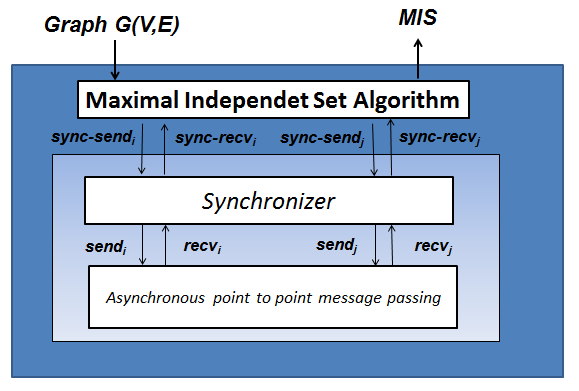
\includegraphics[width=1 \linewidth, height=8cm]{simulation.PNG} 
\caption{Diagram of the simulation of a synchronous distributed systems using synchronizers}
\label{fig:simulation}
\end{figure}



Synchronizers use the local model as well as symmetry breaking algorithms. The local model was used by Awerbuch \cite{awerbuch1985complexity} and previously in \cite{segall1983distributed,gallager1982distributed} among others. Additionally, the messages delay is assumed to be finite but unbounded, and the amount of information carried by messages is limited in the sense that is not expected that processes send messages of unbounded size.

Processes send messages after they receive a pulse or clock in the synchronous model. This pulse represents one-time unit (round) in the synchronous system. The delay of the messages in one round is one unit of time of the global clock.

Because message delay is unbounded, waiting until all messages arrive is not an option to detect if a round has already finished. One approach is send additional messages to achieve synchronization. The notion of safe process was introduced in \cite{awerbuch1985complexity}.



\begin{definition}
\label{def:safe}
A process $p_i$ is said to be safe in a round only after all its messages has been delivered at their destinations.
\end{definition}

An easy solution to detect if a process is safe, it is to force each process to acknowledge every message that receives. If all neighbours of $p_i$ are safe for the round $r$, this means that $p_i$ has received all messages for $r$. In this case, $p_i$ in ready to execute the $r + 1$ round. This property ensures that from the user point of view, the network behaves as a synchronous communication system when it is an asynchronous system. 

The overhead generated by a Synchronizer $S$ with the acknowledgement mechanism is the twice the number of messages of the original algorithm $A$. To compute the total messages and time complexity of a synchronous algorithm, it is necessary to sum the complexity of $A$ and $S$. $T(S)$ and $M(S)$ denote the time and message complexity of $S$ per round respectively. If the synchronizer requires an initialisation phase (for instance, the Beta synchronizer) $T_{init}(S)$ and $M_{init}(S)$ express the message and time complexity of the initialisation phase.  $M(A)$ and $T(A)$ are the time and message complexity of the algorithm $A$. Finally, the total message complexity is represented in the equation \ref{ec:mess} and the time complexity in the equation \ref{ec:time}. 


\begin{equation}
\label{ec:mess}
 T_{tot} = T_{init}(S) + T(A)(1+T(S)) 
\end{equation}

\begin{equation}
\label{ec:time}
M_{tot} = M_{init}(S) + M(A) + T(A)M(S) 
\end{equation}


The two synchronizers presented in the next section are denoted Synchronizer $\alpha$ and Synchronizer $\beta$ \cite{awerbuch1985complexity}, which are a generalisation of the implementation proposed by Gallager in \cite{gallager1982distributed}. These two synchronizers present a trade off on messages and time. Synchronizer $\alpha$ is efficient in time but produce a significant overhead in messages, while Synchronizer $\beta$ has a better performance in communication, but it is worse in time.



\subsection{Alpha Synchronizer}

The Synchronizer $\alpha$ uses the acknowledgement mechanism to detect when a process is safe with respect a one round. A process $p_i$ send an acknowledgement for each message that receives. After $p_i$ received acknowledgements for all its messages, then $p_i$ knows that it is safe for the round $r$. When $p_i$ detect that it's safe, then send a message \textbf{<safe,round>} to all its neighbours. Once $p_i$ learns that all its neighbours are safe, then $p_i$ is ready for a new round.

The code for Synchronizer $\alpha$ is described in the pseudo-code \ref{algorithm:alpha} which was extracted from \cite{attiya2004distributed}.  

\begin{algorithm}
 \caption{Alpha Synchronizer, code for $p_i$ from $i = 1$ to $N$}
 \label{algorithm:alpha} 

\SetAlgoNoLine

Initially \textit{round} = 0 and \newline
\textit{buffer[r], safe[r]} and \textit{ack-missing[r]} are empty for all $r \geq 1$ \newline

\textbf{When} \textit{Synch-}$send_i$ (S) occurs:\newline
$round = round + 1$ \newline
\textit{ack-missing[round]} = {$j:p_j$ is a recipient of a message in S} \newline
enable \textit{Asynch-}$send_i(<m,round>)$  to $p_j$, for each $m \in S$ with recipient $p_j$ \newline

\textbf{When} \textit{Asynch-}$recv_i(<ack,r>)$ from $p_j$ occurs: \newline
add $(m,j)$ to \textit{buffer[r]} \newline
enable $Asynch-send_i(<ack,r>)$ to $p_j$ \newline

\textbf{When} \textit{Asynch-}$recv_i(<ack,r>)$ from $p_j$ occurs: \newline
remove \textit{j} from \textit{ack-missing[r]} \newline
\If{ack-missing[r] = 0}{ 
enable \textit{Asynch-}$send_i(<safe,r>)$ to all neighbours \newline
}

\textbf{When} \textit{Asynch-}$recv_i(<safe,r>)$ from $p_j$ occurs: \newline
add \textit{j} to \textit{safe[r]} \newline
\If{safe[r] includes all neighbours}{
  enable \textit{Synch-}$recv_i(buffer[r])$ \newline
}

\end{algorithm}

The equation \ref{ec:message-alpha} describes the message complexity of Synchronizer $\alpha$ per round. In each round $p_i$ send acknowledgement for each message to all its neighbours, so the complexity is bounded by the number of edges of the network. For this synchronizer, $p_i$ needs one additional time unit to detect that it is safe. Therefore the time complexity is constant (equation \ref{ec:time-alpha}).  

\begin{equation}
\label{ec:message-alpha}
 C(\alpha) = O(E) = O(V^2) 
\end{equation}

\begin{equation}
\label{ec:time-alpha}
 T(\alpha) = O(1) 
\end{equation}


\subsection{Beta Synchronizer}

The Synchronizer $\beta$ is similar to the previous synchronizer. The difference with the Synchronizer $\alpha$ is the safe detection mechanism. This synchronizer needs an initialisation phase in which a rooted spanning tree is constructed over the network topology. A leader $S$ has to be chosen; then the spanning tree is built from the root. 

The acknowledgement mechanism is similar, but instead of $p_i$ informs all its neighbours that it is safe, $p_i$ notify just to its parent in the spanning tree, this process is call convercast. A process $p_i$ is safe when has received the acknowledgement for each message sent in the actual round plus an additional \textbf{<safe,round>} from all its children in the spanning tree. Initially, only processes that are on the bottom of the spanning tree (the leaves) send the message \textbf{<safe,round>}. Progressively, the parents of the leaves send this message to their parents once they are safe until the root receives the safe message. Then, the root broadcast \textbf{OK} on the spanning tree and every process is allowed to pursue with the next round. 

This mechanism blows up the time overhead since the convercast and broadcast act as a global synchronizer with a central leader, the root of the spanning tree. However, $p_i$ only send one safe message instead of sending to all its neighbourhood improving the message overhead of Alpha. The pseudo-code for Beta is described in \ref{algorithm:beta}.


\begin{algorithm}
 \caption{Beta Synchronizer, code for $p_i$ from $i = 1$ to $N$}
 \label{algorithm:beta} 

\SetAlgoNoLine

Compute a rooted spanning tree
Initially \textit{round} = 0 and \newline
\textit{buffer[r], safe[r]} and \textit{ack-missing[r]} are empty for all $r \geq 1$ \newline

\textbf{When} \textit{Synch-}$send_i$ (S) occurs:\newline
$round = round + 1$ \newline
\textit{ack-missing[round]} = {$j:p_j$ is a recipient of a message in S} \newline
enable \textit{Asynch-}$send_i(<m,round>)$  to $p_j$, for each $m \in S$ with recipient $p_j$ \newline

\textbf{When} \textit{Asynch-}$recv_i(<ack,r>)$ from $p_j$ occurs: \newline
add $(m,j)$ to \textit{buffer[r]} \newline
enable-$Asynch-send_i(<ack,r>)$ to $p_j$ \newline

\textbf{When} \textit{Asynch-}$recv_i(<ack,r>)$ from $p_j$ occurs: \newline
remove \textit{j} from \textit{ack-missing[r]} \newline
\If{ack-missing[r] = 0}{ 
enable \textit{Asynch-}$send_i(<safe,r>)$ to my parent in the spanning tree \newline
}
\If{$p_i$ is the root}{ 
enable \textit{Asynch-}$send_i(<go,r>)$ all my childrens in the spanning tree \newline
}

\textbf{When} \textit{Asynch-}$recv_i(<go,r>)$ from $p_j$ occurs: \newline
  enable \textit{Synch-}$recv_i(buffer[r])$ \newline
  enable \textit{Asynch-}$send_i(<go,r>)$ all my childrens in the spanning tree \newline

\end{algorithm}

The diameter of the spanning tree is $N - 1$, so the convercast and broadcast take at most $2N - 2$ time units combined. The initialisation phase only needs to be done one time for each topology, for this reason it is more interesting the overhead $T(\beta)$ and $M(\beta)$. The time and message complexity of the initialisation phase are $T_{init}(\beta) = O(V)$ and $M_{init}(\beta) = O(M + N \log N)$  respectively. Time and message  complexity per synchronous round are expressed in the equations \ref{ec:message-beta} and \ref{ec:time-beta} respectively.

\begin{equation}
\label{ec:message-beta}
 C(\beta) = O(V)
 \end{equation}

\begin{equation}
\label{ec:time-beta}
 T(\beta) = O(V) 
\end{equation}

\subsection{Discussion about Synchronisation techniques}

One synchronizer is efficient in terms of time and the other in term of messages. The same author proposes \cite{awerbuch1985complexity} another synchronizer that tries to get a small overhead in both, the Synchronizer $\gamma$. Essentially, the idea is to generate a spanning forest of the graph and run Beta within each tree and Alpha between trees. If there are not too many adjacent trees, the messages overhead is similar to the Beta Synchronizer. The time cost is proportional to the depth of the trees. In some special cases  (depending on the topology of the graph, for instance, a ring of k-cliques \cite{lynch1996distributed}), the Gamma Synchronizer can present a similar cost to the original synchronous algorithm. However, it is also possible the need of tuning the spanning forest for some types of graphs. Besides, the Gama Synchronizer is more complex in terms of implementation and initialisation phase.

All these synchronizers require that the entire network participates in the synchronisation process, even if some process has no message for the round. The problem is when $p_i$ do not send any messages in one round, then any process $p_j$ that is a neighbour of $p_i$ cannot deduce this situation because the delays in asynchronous networks are unbounded. In consequence, the use of a timer is not useful. One solution is to send dummy messages to keep the synchronisation. As a result, the overhead is always linear on the number of processes. Awerbuch and Peleg proposed in \cite{awerbuch1990network} a poly-logarithmic overhead synchronizer based on involving only the relevant portion of the topology in the synchronisation process. However, it is possible that the synchronizer requires high space complexity.

Another approach for dynamic networks is for each process calculate the active neighbours before the start of the rounds, and then apply a simple synchronizer, Alpha for instance. This strategy study in \cite{AspnesW2007} requires additional messages to calculate active processes, but no dummy messages are needed. 

For the simulations in this project, besides the Beta and Alpha Synchronizers, a global synchronisation mechanism is used, similar to the approach for dynamic networks. A master process $M$ is required to control the synchronisation between every active process on the network.  Each process must inform $M$ that has finished the computation for the round $r$ and then $M$ is in charge of notifying active processes that are allow to start the $r + 1$ round. This mechanism generates a lot of computation in the master process, however, no unnecessary message is sent by inactive process. Besides the Beta and Alpha synchronizers, a global synchronisation mechanism, similar to the approach for dynamic networks, is tested in the simulations. 

In the global synchronisation, a master process $M$ controls the the rounds execution for all processes in the network. Each active $p_i$ must inform $M$ that has finished the computation for the round $r$. When all processes inform the finalisation of the round, then $M$  notify to the active processes that they are allowed to start the $r + 1$ round. $M$ can decide which processes are going to be active for the next round and only these processes receive the notification. Before the start of a new round, each active $p_i$ has to send request messages to its neighbour to detect which processes are active for the current round. This mechanism generates a lot of messages to the master process and creates a bottle neck on it. However, there are no extra messages sent by inactive processes or to them.   

In the case of the Distributed Maximal Independent Set problem, especially with the algorithms explained in the previous section, this behaviour is desirable because many processes become inactive very quickly. These three techniques are used to simulate a synchronous communication for the \textit{MIS} algorithm. The analysis of the trade-off among them is presented in section \ref{chap:6}.




